\chapter{Solving the initial issues}\label{chap:chap3}

\epigraph{``Much of the excitement we get out of our work is that we don't really know what we are doing''}{\textit{Edsger W. Dijkstra}}

\paragraph{}
In this short chapter we will present the fixes for the initial bugs in the logic of the simulator discussed in Section \ref{chap:chap1outsidelook} that were performed in order to bring it to an acceptably working state. In the end, an additional fix will be presented concerning the datapath visualization. This last fix was performed near the end of the thesis' work, but, since it doesn't per se represent an addition to the simulator, it was decided to include it in this chapter. Both in this and the following chapters, the source code will not be presented in its original form, but slightly cleaned up and simplified to highlight only the essential components.

\section{Fixing the comparison behavior}
\paragraph{}
As we have showcased in Section \ref{chap:chap1outsidelook}, the simulator seems unable to perform comparisons in the correct way, and ignores a conditional jump that it should have instead followed. Figure \ref{fig:flagbug2} shows again the aforementioned execution flow.
\begin{figure}[H]
	\centering
	\subfigure[X0 < X1]{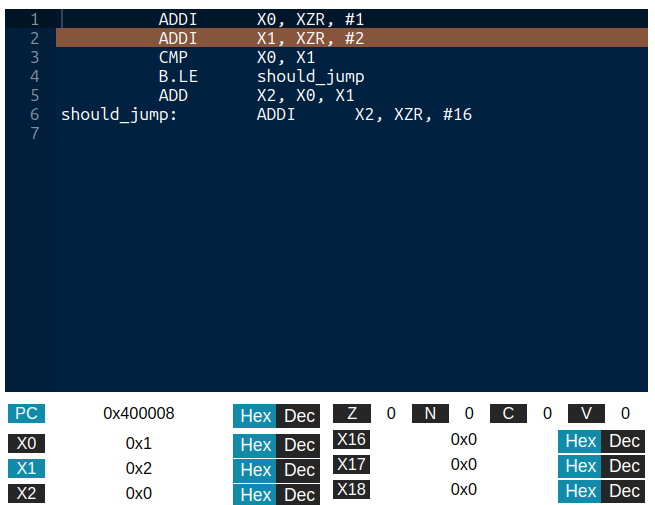
\includegraphics[width=.45\textwidth]{img/cmp_bug_1.png}}
	\subfigure[Comparison sets the flags incorrectly.]{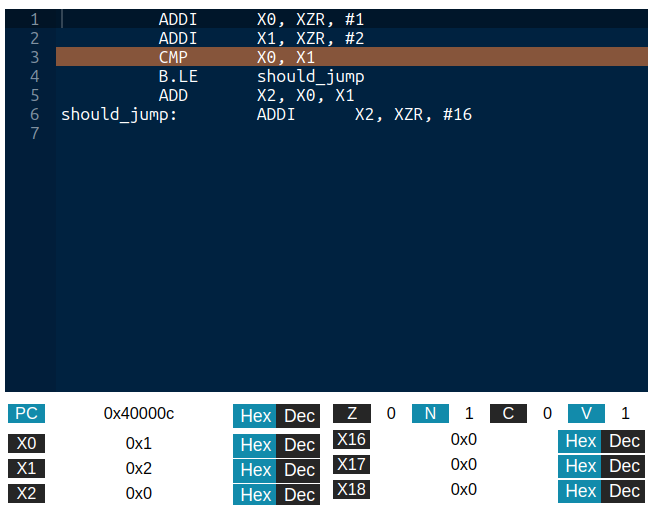
\includegraphics[width=.45\textwidth]{img/cmp_bug_2.png}}
	\subfigure[Less-or-equals jump doesn't happen.]{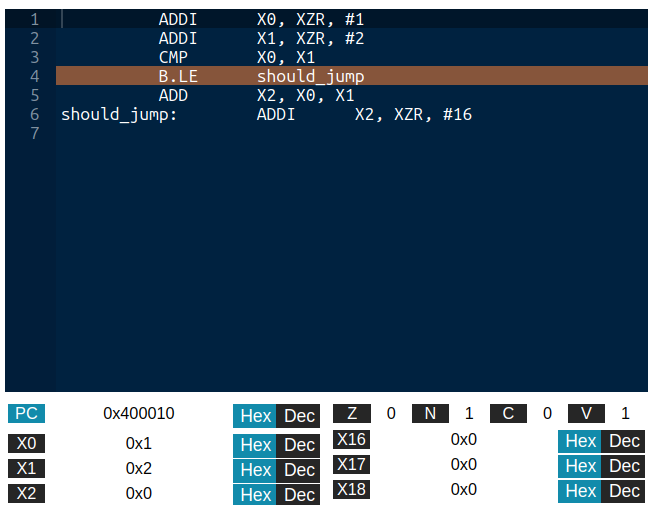
\includegraphics[width=.45\textwidth]{img/cmp_bug_3.png}}
	\subfigure[Wrong instruction executed.]{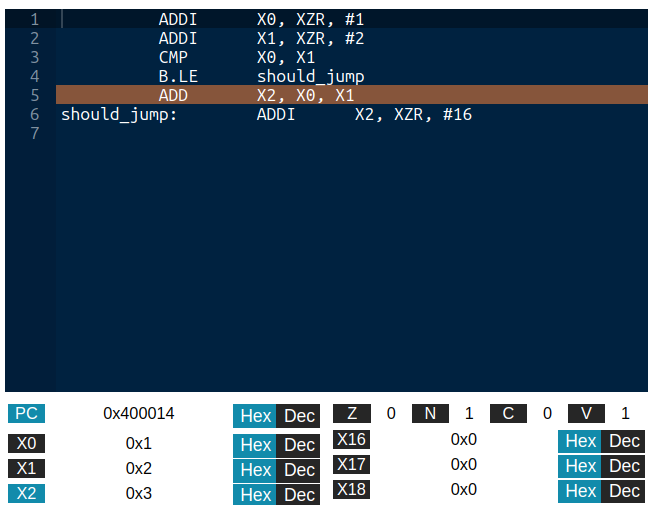
\includegraphics[width=.45\textwidth]{img/cmp_bug_4.png}}
	\caption{Comparisons do not set the correct flags and thus fail.}
        \label{fig:flagbug2}
\end{figure}
First thing to note is that \verb|CMP| is a \emph{pseudo-instruction}. This term refers to virtual instructions that have their own mnemonic and syntax, but under the hood are implemented using one or more ``real'' instructions. In short, they are useful aliases for the developers. The overview of the codebase in Section \ref{chap:chap1insidelook} directs us to look into the \verb|Decoder.java| class. Here we find that the developers implemented the \verb|CMP| instruction following the way it's described in the LEGv8 specification, namely as an alias for the \verb|SUBS| instruction. 
This last instruction performs the integer subtraction between two registers, writes the result to a third one, and sets the flag registers according to the criteria listed in Section \ref{chap:chap1registers}. Since what we are interested in is not the actual subtraction, but to compare the two registers, \verb|CMP| only has two arguments instead of three, and it gets translated to a \verb|SUBS| instruction in which the destination register of the subtraction is \verb|XZR| (i.e. \verb|X31|, the constant zero register), as shown in Listing \ref{lst:cmp}. 
\begin{lstlisting}[float, caption={The CMP mnemonic being translated into a SUBS instruction}, label={lst:cmp}]
case CMP :
		return new Instruction(Mnemonic.SUBS, ...);
...
private static int[] decodeCMPArgs(ArrayList<String> args) {
	int[] operands = new int[3];
	operands[0] = decodeRegister("XZR");
	operands[1] = decodeRegister(args.get(0));
	operands[2] = decodeRegister(args.get(1));
	return operands;
}
\end{lstlisting}
After performing the comparison through \verb|SUBS|, no registers are written to, and the flags are set. At this point, to determine the outcome of a conditional jump instruction (such as in this case \verb|B.LE|, meaning branch if less or equal), the flags are read and interpreted, and the jump follows accordingly. Figure \ref{fig:condjumpflags} shows the jump conditions when the flags are set by a subtraction.
\begin{figure}
    \centering
    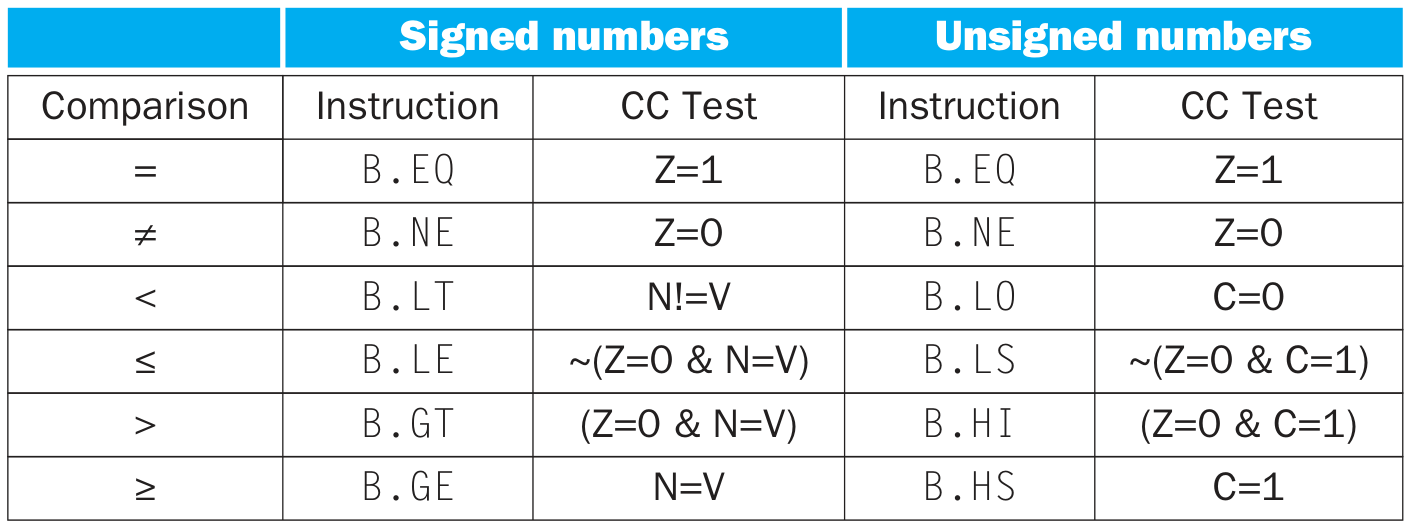
\includegraphics[width=1\linewidth]{img/condjumpflags.png}
    \caption{Conditions for each conditional jump instruction in the case of subtraction. From \emph{Computer Organization and Design (ARM Edition)} \cite{patterson2016computer} p. 98}
    \label{fig:condjumpflags}
\end{figure}
From the previous description, two options present themselves: either \verb|SUBS| sets the wrong flags, or \verb|B.LE| interprets them incorrectly. Let's look at \verb|SUBS| in Listing \ref{lst:subs}.
\begin{lstlisting}[float, caption={SUBS' implementation}, label={lst:subs}]
private void SUBS(int destReg, int op1Reg, int op2Reg) {
    registerFile[destReg] = registerFile[op1Reg] - registerFile[op2Reg];
    SUBSetFlags(result, registerFile[op1Reg], registerFile[op2Reg]);
}
\end{lstlisting}
The subtraction seems to work fine, but the actual flag-setting is being performed by a helper function \verb|SUBSetFlags|, shown in Listing \ref{lst:subsetflagsold}.
\begin{lstlisting}[float, caption={Function that sets SUBS' flags}, label={lst:subsetflagsold}]
private void SUBSetFlags(long result, long op1, long op2) {
	ADDSetFlags(result, op1, op2);
}
\end{lstlisting}
As we can see, the function itself makes use of  \verb|ADDSetFlags|, a function responsible for setting the flags for the addition instructions. This is strange, because \verb|ADDSetFlags| is being called with the same arguments as \verb|SUBSetFlags| even though the criteria for setting the flags in the case of an addition are different than with subtraction. We remember, though, that we can interpret a subtraction as an addition and vice versa, so all that is needed to fix this behavior is to call \verb|ADDSetFlags| with the two's complement of \verb|op2| as depicted in Listing \ref{lst:subsetflagsnew}, thus eliminating a need for two implementations.
\begin{lstlisting}[float, caption={The fixed function}, label={lst:subsetflagsnew}]
private void SUBSetFlags(long result, long op1, long op2) {
    ADDSetFlags(result, op1, |(~(op2)+1)|);
}
\end{lstlisting}
Testing the various jump conditions with \verb|CMP| after this change gives positive results, proving that \verb|ADDSetFlags| was implemented correctly and this was the source of the issue.
\section{Fixing the branch and link behavior}
\paragraph{}
The other bug that was discussed, concerned an incorrect behavior when performing function calls. The purpose of the branch and link instruction \verb|BL| is to jump to a label representing a function or subroutine, and then, through a branch return \verb|BR| instruction, go back to where the function was originally called and resume execution. To achieve this, as opposed to a normal branch, two additional steps have to be performed. Firstly, the program counter pointing to the original function call needs to be saved somewhere. This is performed automatically by the \verb|BL| instruction by saving the address to the appropriately named \emph{link register} \verb|LR| (i.e., \verb|X30|). Secondly, the \verb|BR| instruction needs to be told to jump back to the aforementioned address. Unlike with \verb|BL|, \verb|BR| takes a register as an argument and thus doesn't automatically assume it needs to be \verb|LR|, meaning we can in theory tell it to jump to user-defined locations in the source code. The usual case, though, is to tell the \verb|BR| to jump to the instruction pointed by \verb|LR|. As was the case in the last section, either the \verb|BL| instruction sets the wrong return address, or the \verb|BR| instruction somehow interprets it incorrectly. We can see in Listing \ref{lst:blold} how \verb|BL| is implemented in \verb|CPU.java|, and immediately we can spot the problem.
\begin{lstlisting}[float, caption={BL's implementation}, label={lst:blold}]
private void BL(int branchIndex) {
    instructionIndex = branchIndex;
    registerFile[LR] = instructionIndex * INSTRUCTION_SIZE + Memory.TEXT_SEGMENT_OFFSET;
}
\end{lstlisting}
\verb|instructionIndex| first  gets updated with the address of the function, and \emph{then} gets written to the \verb|LR| register, meaning that \verb|LR| contains the address of the function's label and not the current value of the program counter. Other than that, the code is correct, and all that is needed is to invert the order of operation as shown in Listing \ref{lst:blnew}.
\begin{lstlisting}[float, caption={BL's correct implementation}, label={lst:blnew}]
private void BL(int branchIndex) {
    |registerFile[LR] = instructionIndex * INSTRUCTION_SIZE + Memory.TEXT_SEGMENT_OFFSET;|
    |instructionIndex = branchIndex;|
}
\end{lstlisting}
\section{Realigning the stack}
\paragraph{}
As mentioned in Chapter \ref{chap:chap1}, the stack grows from the top of the memory following an address called the \emph{stack pointer} (SP). The authors of the textbook \cite{patterson2016computer} specify that its starting value must be \emph{quadword aligned}, meaning that, in LEGv8, it must be a multiple of 128. For some reason though, the authors set the stack pointer's initial value to $\verb|7ffffffffc|_2$, which is not quadword aligned. It has thus been chosen to adjust this value to $\verb|8000000000|_2$, fixing the problem.
\section{Fixing a datapath visualization bug}
\paragraph{}
A bug that was addressed much later during this thesis' work, was first pointed out on the project's GitHub page \cite{legv8simARMrepogit} under the Issues section by user \verb|aaarbk|. The bug consisted in the \verb|Memread| and \verb|Memwrite |signals being given the wrong values in the datapath visualization for the single cycle execution mode. Namely, they appear to behave oppositely than expected, with \verb|Memwrite| being 0 when writing to the memory and \verb|Memread| being 1. The code responsible, shown in Listing \ref{lst:memreadold}, is divided between \verb|SingleCycleVis.java| and \verb|ControlUnitConfiguration.java|.
\begin{lstlisting}[float, caption={The old Memread signal logic}, label={lst:memreadold}]
ctx.fillText(c.memRead, ...);
ctx.fillText(c.memWrite, ...);
...
/**
* @param reg2Loc		the value of the Reg2Loc control signal
* @param uncondBranch	the value of the UncondBranch control signal
* @param flagBranch	the value of the FlagBranch control signal
* @param zeroBranch	the value of the ZeroBranch control signal
* @param memRead		the value of the MemRead control signal
* @param memToReg		the value of the MemToReg control signal
* @param memWrite		the value of the MemWrite control signal
* @param flagWrite		the value of the FlagWrite control signal
* @param aluSrc		the value of the ALUSrc control signal
* @param aluOp			the value of the ALUOp control signal
* @param regWrite		the value of the RegWrite control signal
*/
...
RM_LOAD(..., false, true, true, ...),
\end{lstlisting}
Due to the behavior of the bug, it's easy to see that in \verb|ControlUnitConfiguration.java|, the \verb|Memwrite| and \verb|Memread| signals (namely, the 5th and 7th argument) for  \verb|RM_LOAD| type instructions are swapped and, similarly, in \verb|SingleCycleVis.java| \verb|c.memRead| and \verb|c.memWrite| are swapped too. Listing \ref{lst:memreadnew} shows the correct code.
\begin{lstlisting}[float, caption={The fixed Memread signal logic}, label={lst:memreadnew}]
ctx.fillText(|c.memWrite|, ...);
ctx.fillText(|c.memRead|, ...);
...
RM_LOAD(..., |true|, true, |false|, ...),
\end{lstlisting}
This concludes the discussion of the original bugs present in the simulator that have been fixed during this thesis' work.
\section{Conclusions}
\paragraph{}
Fortunately, the bugs discussed, at least the first two, were as critical as they were simple to fix. Both of them were probably a result of the developer's distraction, but greatly impacted the viability of the simulator. While this chapter talked about changes of the original code that simply fixed undesired behavior, the next chapter will present all the notable additions that have been made to the simulator, expanding on its original design.